\documentclass[12pt, bibliography=totoc]{scrartcl}
\usepackage[headsepline,automark]{scrlayer-scrpage} %Trennlinie an Kopfzeile
%\usepackage{scrheadings}
\clearpairofpagestyles
\lohead{\rightmark}
%\renewcommand{\partmark}[1]{\relax}% \part daran hindern, den Kolumnentitel zu löschen
\ohead[]{\pagemark}
%\ofoot*{\pagemark}
%%Kopfzeile
\usepackage{txfonts} %für times new roman
%\usepackage{helvet} %für arial, dann aber 11pt
\usepackage[a4paper, left=2cm, right=2.5cm]{geometry}
\usepackage[onehalfspacing]{setspace}
%\usepackage{apacite}
\usepackage{wasysym}
\usepackage{mbenotes}
\usepackage{rotating}
\usepackage{amsmath}
\usepackage{amssymb}
\usepackage{float}
%\usepackage{caption}
\usepackage[T1]{fontenc}
\usepackage[utf8]{inputenc}
%\usepackage{todonotes}
\usepackage{enumitem}
%\uespackage{caption}
%\usepackage[bf]{caption}
%\renewcommand{\captionfont}{\small\slshape}
%\renewcommand{\figurename}{Abb.}
%\renewcommand{\thefigure}{\arabic{section}.\arabic{figure}}
%\makeatletter \@addtoreset{figure}{section} \makeatother
%\captionsetup[figure]{skip=1pt}
\usepackage{tabularx}
\usepackage{pdfpages}
\usepackage{array}
\usepackage{hyperref}
\usepackage{threeparttable} %fußnoten unterhalb tabelle
\usepackage{booktabs} % fuer schone Tabellen
\usepackage{rotating} % um tabellen auf quer drehen zu koennen http://www.golatex.de/kann-man-tabellen-im-querformat-darstellen-t2003.html
%\newcolumntype{C}[1]{>{\centering\arraybackslash}p{#1}} %Spalten mit fester breite zentriert
%\newcolumntype{L}[1]{>{\raggedright\arraybackslash}p{#1}} %Spalten mit fester breite linksbündig
%\newcolumntype{Y}{>{\small\raggedright\arraybackslash}X}
%\newcolumntype{C}{>{\small\centering\arraybackslash}X}
\usepackage{graphicx}
%\usepackage[german]{babel}
\usepackage{typearea}
%für Randbemerkungen, sehr nützlich:
\usepackage{xargs}                      % Use more than one optional parameter in a new commands
\usepackage[pdftex,dvipsnames]{xcolor}
\usepackage[colorinlistoftodos,prependcaption,textsize=tiny]{todonotes}
\newcommandx{\unsure}[2][1=]{\todo[linecolor=red,backgroundcolor=red!25,bordercolor=red,#1]{#2}}
\newcommandx{\change}[2][1=]{\todo[linecolor=blue,backgroundcolor=blue!25,bordercolor=blue,#1]{#2}}
\newcommandx{\info}[2][1=]{\todo[linecolor=OliveGreen,backgroundcolor=OliveGreen!25,bordercolor=OliveGreen,#1]{#2}}
\newcommandx{\improvement}[2][1=]{\todo[linecolor=Plum,backgroundcolor=Plum!25,bordercolor=Plum,#1]{#2}}
\newcommandx{\thiswillnotshow}[2][1=]{\todo[disable,#1]{#2}}
% erklaerung siehe hier http://tex.stackexchange.com/questions/9796/how-to-add-todo-notes

%hat prima funktioniert:
\usepackage[style=apa,backend=biber]{biblatex}
\usepackage[american,ngerman]{babel}
\DeclareLanguageMapping{ngerman}{ngerman-apa}
\usepackage[babel,german=guillemets]{csquotes}
%\bibliographystyle{apacite}
%nach part fängt section wieder mit eins an alte Gestaltung
%\makeatletter
%\@addtoreset{section}{part}
%\makeatother
%\renewcommand*{\partformat}{\thepart}{}
%\renewcommand*{\partheadmidvskip}{\nobreak\enskip}
%\bibliography{/Users/iNge/Dropbox/Biblio/ingesbibneu}
\bibliography{/Users/iNge/Dropbox/Biblio/library}
%\bibliography{library}




\begin{document}
\renewcommand\finalandcomma{\addcomma}

\begin{titlepage}
\thispagestyle{empty}
\begin{center}
\color{blue}\Large{Fernuniversität Hagen}\\
\end{center}


\begin{center}
\Large{Bildung und Medien: eEducation}
\end{center}
\begin{verbatim}



\end{verbatim}
\begin{center}
\textbf{\Large{Kommentierte Bibliographie zum Thema Online-Lernen}}
\end{center}
\begin{verbatim}

\end{verbatim}
\begin{center}
\textbf{Fakultät Kulturwissenschaften}
\end{center}
\begin{verbatim}










\end{verbatim}

\begin{flushleft}
\begin{tabular}{lll}
\textbf{Studiengang:} & & MA Bildung und Medien: eEducation\\
& & Modul 2: Anwendungsbezogene Bildungsforschung\\
& & \\
& & \\
\textbf{eingereicht von:} & & {\color{magenta} Inge Koch-Meinass \flq{}ingekoch@mac.com\frq{}}\\
& & {\color{magenta}Matrikelnr.: 123456 }\\
& & \\
\textbf{eingereicht am:} & & 06. November 2015\\
& & \\
& & \\
%\textbf{Betreuer:} & & Herr Prof. Dr. J. A. Müller
\end{tabular}
\end{flushleft}

% das ist wohl jetzt das Ende des Dokumentes
\end{titlepage}


%% das Papierformat zuerst
%\documentclass[a4paper, 11pt]{article}

% deutsche Silbentrennung
%\usepackage[ngerman]{babel}
%\usepackage{color} \color{blue}
% wegen deutschen Umlauten
%\usepackage[utf8]{inputenc}

% hier beginnt das Dokument
%\begin{document}

\begin{titlepage}
\thispagestyle{empty}
\begin{center}
\color{blue}\Large{Fernuniversität Hagen}\\
\end{center}


\begin{center}
%\Large{Bildung und Medien: eEducation}
\end{center}
\begin{verbatim}



\end{verbatim}
\begin{center}
\textbf{\Large{Kommentierte Bibliographie zum Thema Online-Lernen}}
\end{center}
\begin{verbatim}

\end{verbatim}
\begin{center}
%\textbf{im Studiengang Wirtschaftsinformatik}
\end{center}
\begin{verbatim}











\end{verbatim}

\begin{flushleft}
\begin{tabular}{lll}
\textbf{Studiengang:} & & MA Bildung und Medien: eEducation\\
& & Modul 2: Anwendungsbezogene Bildungsforschung\\
& & \\
& & \\
\textbf{eingereicht von:} & & {\color{magenta} Inge Koch-Meinass \flq{}ingekoch@mac.com\frq{}}\\
& & {\color{magenta}Matrikelnr.: 9650962 }\\
& & \\
\textbf{eingereicht am:} & & 06. November 2015\\
& & \\
& & \\
%\textbf{Betreuer:} & & Herr Prof. Dr. J. A. Müller
\end{tabular}
\end{flushleft}

% das ist wohl jetzt das Ende des Dokumentes
\end{titlepage}

\listoftodos{Gesammelte Unklarheiten}
\tableofcontents
%\listoftables
\setcounter{page}{1}
%\thispagestyle{empty}
\pagebreak

\section{Einleitung}\label{einleitung}

Der beruflichen Weiterbildung kommt eine immer größeere Bedeutung zu,
die Notwendigkeit zum lebenslangen Lernen ist in vielen Berufssparten
da. Das immer größere Lernpensum, kann nicht ausschließlich in
Präsenzveranstaltung gelehrt werden, sondern viel mehr gilt es von Zeit
und Ort unabhängige Lernmöglichkeiten zu schaffen. Digitale
Lernplattformen leisten hier einen wichtigen Beitrag und können je nach
didaktischer Aufbereitung, selbstorganisiertes, konstruktuvistisches und
damit nachhaltiges Lernen fördern.

Die vorliegende Arbeit befasst sich mit der Evaluation einer beruflichen
Weiterbildung, die als Blended Learning Kurs für
FrühpädagogInnen\footcite{Der Begriffe FrühpädagogInnen, schließt alle im Kitabereich tätigen Fachkräfte ein}
konzipiert wurde. Inhalt der Weiterbildung ist das kennenlernen und
umsetzen können des Early-Excellence Konzept, ein Ansatz mit dem
Bildungs- und Orientierungspläne der Bundesländer umgesetzt werden
können. Mit Hilfe eines standardisierten Fragebogens wird versucht den
durch die Weiterbildung gewonnen Zuwachs an Kompetenz zu bestimmen. Es
wird einmal das Weiterbildungsangebot insgesamt und zum anderen der
Einfluss der digitalen Lernplattform betrachtet.

\section{Theorierahmen}\label{theorierahmen}

Der der Untersuchung zugrundeliegende Theorierahmen umfasst die
Förderung von Handlungskompetenz Thema Erwachsenenbildung
\unsure{berufliche Weiterbildung} und Blended Learning Verfahren
auseinander.

\subsection{Erwachsenendidaktik}\label{erwachsenendidaktik}

Da die Weiterbildung sich an (ältere) Erwachsene richtet und sehr
prozesshaft aufgebaut, wird hier das Lernen von Erwachsenen anhand des
\enquote{Transformational Learning} erklärt. Jack Mazirow gilt als
bedeutenster Verteter und Begründer dieser Theorie. Diese Theoerie geht
davon aus, dass Erwachsene

\subsection{Blended Learning}\label{blended-learning}

Im folgenden soll der Begriff des Blended Learning und was im Rahmen
dieser Arbeit darunter zu verstehen erläutert werden. Direkt übersetzt
bedeutet Blended Lerning \enquote{vermischtes Lernen}. Das heißt es
handelt sich bei dieser Lernform um ein Lehr-Lernsetting, dass sowohl
klassisches Face-to-Face-Lernen, als auch eLearning beinhaltet. Die
verschiedenen Lernangebote stehen sich nicht als entweder oder
gegenüber, sondern als sich ergänzend.
\texcite[3]{kerres2001multimediale} betont \enquote{dass die besondere
Qualität und auch Effizienz eines Lernangebotes vor allem in der
Kombination von Elementen unterschiedlicher methodischer und medialer
Aufbereitung zum Tragen kommt}. Blended Learning Konzepte gibt es schon
seit vielen Jahren und sie werden sowohl in Schulen und Hochschulen ,
als auch in beruflichen Weiterbildungsmaßnahmen eingesetzt. Elearning
Angebote wurden in Deutschland nur sehr zögerlich angenommen, es
überwiegen in weiten Bereichen noch traditioneller Unterricht. Aus
dieser Situation heraus bot es sich an eine Lernform zu benutzen, die
traditonelle und neuzeitliche, digitale Lernformen verbindet
\parentcite{Maihack2015}. Für den Einsatz von Blended Learning sprechen
nach \textcite{thomas2000evaluating} zahlreiche Gründe: * Orts- und
Zeitunabhängigkeit

\begin{itemize}
\item
  Leichte Aktualisierbarkeit
\item
  Lerner haben viel Kontrolle: sie können wählen, was sie wann lernen,
  können auf bereits durchgenommenes Material zugreifen usw.
\item
  Viele Möglichkeiten der Interaktion
\item
  Es können beliebig viele Personen am Kurs teilnehmen
\end{itemize}

Die Form des hybriden Lernens erlaubt es, Vorteile von digitalem Lernen
(selbstorganisiert, zeit- und ortsunabhängig, ) und Vorteile von
traditionellem Lernen (sich kennen lernen, Gruppen bilden, Motivation
\ldots) zu kombinieren \textbackslash{}parentcite\{Zumbach2010).
Zugleich können natürlich auch Nachteile verstärkt werden und z.B. die
Lernerdisziplin abnehemen. Umso wichtiger ist es das Format Blended
Learning so umzusetzen, dass eine optimale Kombination der Lernformen
möglich wird.

Es sei angemerkt, dass es sowohl verschiedene Begriffe, als auch
verschiedene Definitionen von Blended Learning gibt. Neben Begriffen wie
integrated Learning, flexible Learning usw. wird es im deutschen
Sprachraum oft auch als \enquote{Hybrid Teaching} benannt
\parencite{Oliver2005,kerres2001multimediale }. Hier meint Blended
Learning, die sich ergänzende Kombination von verschiedenen Medien,
nämlich traditionellem Präsenzlernen und eLearning in Form einer
Moodle-Lernplattform.

\subsection{Begriffliche Definitionen oder aktueller
Forschungsstand}\label{begriffliche-definitionen-oder-aktueller-forschungsstand}

Blended Learning, Erwachsenenbildung

\subsection{Beschreibung der zu untersuchenden Kompetenzen oder
Meßgröße}\label{beschreibung-der-zu-untersuchenden-kompetenzen-oder-meuxdfgruxf6uxdfe}

\enquote{Die gegenwärtige Begriffsdefinition verweist da- bei vermehrt
auf differente Lehr- und Lernarrangements, denen keine fundierten empi-
rische Studien zugrunde liegen, die mediale und traditionelle
Lernmodelle untersuchen, umso zu einer allgemeingültigen Definition von
Blended Learning beizutragen. Dies liegt mitunter daran, dass die
Transparenz der Grenzen zwischen Präsenzveranstal- tungen und
Onlinesequenzen in der Praxis nicht eindeutig zu identifizieren sind
(vgl. Kraft o.J.; Häfele/Maier-Häfele 2004). Diesbezüglich wird
E-Learning als Bestandteil von Blended Learning angesehen und ist
demzufolge stets miteinbegriffen was auch dieser Arbeit zugrunde liegt
(vgl. Bruns 2006). Lernplattformen}\textcite{Maihack2015}
\improvement{hieraus was entnehmen, es ist wichtig für die Diskussion der Ergebnisse}

\begin{itemize}
\tightlist
\item
  Handlungskompetenz Die Handlungskompetenz kann nach Erpenbeck
  definiert werden als: \info{aus dem dicken Buch was schönes zitieren}
  Besonders in der Erwachsenenbildung geht es nicht vorrangig darum
  abrufbares Wissen zu vermehren, sondern vielmehr liegt der Schwerpunkt
  darauf, durch das neue Wissen handlungsfähig zu werden:
  \unsure{irgendein Zitat mit komplexem lernen}
  \improvement{diese drei Punkt mit Text und Leben füllen und tapfer bleiben}
  Die Effizienz dieses Lernansatzes wird mittels der Veränderung der
  Handlungskompetenz erfasst. Die Handlungskompetenz setzt sich nach
  \textcite{ErpenbeckRosenstiel200305} aus folgenden Kompetenzen
  zusammen:
\end{itemize}

\begin{enumerate}
\def\labelenumi{\arabic{enumi}.}
\tightlist
\item
  Personale Kompetenzen: Diese Kompetenz beschreibt, z.B.:
\end{enumerate}

\begin{itemize}
\item
  Fähigkeit selstorganisiert zu ahndeln
\item
  Selbsteinschätzung
\item
  Produktive Einstellungen
\item
  Motive, Selbstbilder, Werte
\end{itemize}

\% Hier dann alles zum Thema Operationalisierung

\subsection{Inhalte der Weiterbildung}\label{inhalte-der-weiterbildung}

\subsection{Aufbau der Lernplattform}\label{aufbau-der-lernplattform}

\section{Methoden}\label{methoden}

\subsection{Forschungsfrage und
Hypothesen}\label{forschungsfrage-und-hypothesen}

\subsection{Studiendesign}\label{studiendesign}

\begin{itemize}
\tightlist
\item
  Ziel der Evaluation
\item
  formativ
\item
  natürliche Gruppe
\item
  deskriptive Auswertung univariat
\item
  Darstellung der Ergebnisse anhand von Häufigkeiten
\item
  MW, Median, Modal, Streuung
\item
  schriftliche Befragung, vollstandardisiert, alle Teilnehmer,
  Selbseinschätzung
\end{itemize}

\subsection{Messinstrument}\label{messinstrument}

\subsection{Messinstrument}\label{messinstrument-1}

\subsection{Pretest des Fragebogens}\label{pretest-des-fragebogens}

Nach Entwurf des Fragebogens wurde dieser einem Pretest unterzogen. Es
gab 8 Teilnehmer, die durchschnittlcihe Verweildauer betrug ca. 5
Minuten. Die Reliabilität wurde mittels Cronbachs alpha ermittelt
(\textcite{Wassa}) Er ergab für die einzelnen Kompetenzen Werte zwischen
0.72 und 0.98., was als gut bis sehr gut anzusehen ist.

\section{Ergebnisse}\label{ergebnisse}

Die Ergebnisse werden anhand der Summenwerte der einzelnen Kompetenzen
beschrieben. Die Summenwerte setzen sich aus den einzelnen Itembaterrien
zusammen. Die Fachkompetenz und die Personalkompetenz wurde mit je fünf
Items abgefragt. Die Summenwerte wurden in die Klassen
0-5,5-10,10-15,15-20 und 20-25 eingeteilt. Die Methodenkompetenz und die
Kommunikationskompetenz wurde mit je vier Items abgefragt und die
Ergebnisse wurden wie folgt klassifiziert: 0-4,4-8,8-12,12-16,16-20. Es
ergeben sich für jede Kompetenz fünf Klassen, die entprechend der
Likertskala als keinen, geringen, mittleren, hohen und sehr hohen
Kompetenzzuwachs bewertet werden.

\begin{itemize}
\tightlist
\item
  Fachkompetenz Die Häufigkeitstabelle zeigt, dass bei keinem Teilnehmer
  der Zuwachs an Handlungskompetenz als garnicht oder gering
  eingeschätzt wurde. 75 \% der Teilnehmer schätzen dagegen ihren Zuwchs
  an Fachkompetenz als sehr hoch ein.
\end{itemize}

\begin{table}[H]
\centering
\caption{Häufigkeitstabelle Fachkompetenz}
\begin{tabular}{rrrr}
  \hline
 & absolut & Prozent & kumuliert \\
  \hline
(0,5] & 0.00 & 0.00 & 0.00 \\
  (5,10] & 0.00 & 0.00 & 0.00 \\
  (10,15] & 1.00 & 8.33 & 8.33 \\
  (15,20] & 2.00 & 16.67 & 25.00 \\
  (20,25] & 9.00 & 75.00 & 100.00 \\
   \hline
\end{tabular}
\end{table}\begin{figure}[H]
\centering
\includegraphics{Anhang/FKHIST.png}
\caption{Histogramm Fachkompetenz}
\end{figure}

\begin{table}[H]
\centering
\caption{Lage- und Streumaße Fachkompetenz}
\begin{tabular}{rrrrrrrr}
  \hline
  N & Minimum & Maximum & Mittelwert & Median & Modus & SD & Varianz \\
  \hline
 12.00 & 14.00 & 25.00 & 20.58 & 21.00 & 5.00 & 3.03 & 9.17 \\
   \hline
\end{tabular}
\end{table}

\begin{itemize}
\tightlist
\item
  Methodenkompetenz Bei der Methodenkompetenz wurde der Zuwachs von
  keinem Teilnehmer auf Null, aber von drei Teilnehmer als gering
  eingeschätzt. Knapp zweidrittel der Teilnehmer (ca 59\%) schätzen
  ihren methodischen Kompetenzzuwachs auf mittel ein, etwa 17\% auf
  hoch.
\end{itemize}

\begin{table}[H]
\centering
\caption{Häufigkeitstabelle Methodenkompetenz}
\begin{tabular}{rrrr}
  \hline
 & absolut & Prozent & kumuliert \\
  \hline
(0,5] & 0.00 & 0.00 & 0.00 \\
  (5,10] & 3.00 & 25.00 & 25.00 \\
  (10,15] & 7.00 & 58.33 & 83.33 \\
  (15,20] & 2.00 & 16.67 & 100.00 \\
  (20,25] & 0.00 & 0.00 & 100.00 \\
   \hline
\end{tabular}
\end{table}\begin{figure}[H]
\centering
\caption{Histogramm Methodenkompetenz}
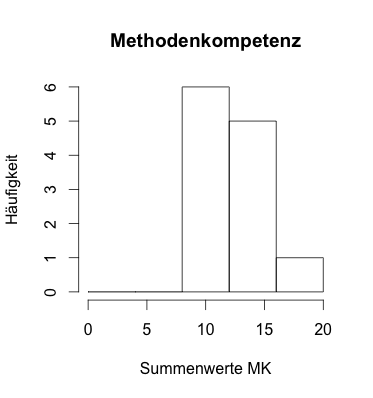
\includegraphics[width=0.33\textwidth]{Anhang/MKHist.png}
\end{figure}

\begin{table}[H]
\centering
\caption{Lage- und Streumaße Methodenkompetenz}
\begin{tabular}{rrrrrrrr}
  \hline
  N & Minimum & Maximum & Mittelwert & Median & Modus & SD & Varianz \\
  \hline
  12.00 & 10.00 & 17.00 & 12.83 & 12.50 & 3.00 & 2.41 & 5.79 \\
   \hline
\end{tabular}
\end{table}

\begin{itemize}
\tightlist
\item
  Personalkompetenz
\end{itemize}

\begin{table}[H]
\centering
\caption{Häufigkeitstabelle Personalkompetenz}
\begin{tabular}{rrrr}
  \hline
 & absolut & Prozent & kumuliert \\
  \hline
(0,5] & 0.00 & 0.00 & 0.00 \\
  (5,10] & 0.00 & 0.00 & 0.00 \\
  (10,15] & 1.00 & 8.33 & 8.33 \\
  (15,20] & 8.00 & 66.67 & 75.00 \\
  (20,25] & 3.00 & 25.00 & 100.00 \\
   \hline
\end{tabular}
\end{table}

\begin{figure}[H]
\centering
\caption{Histogramm Methodenkompetenz}
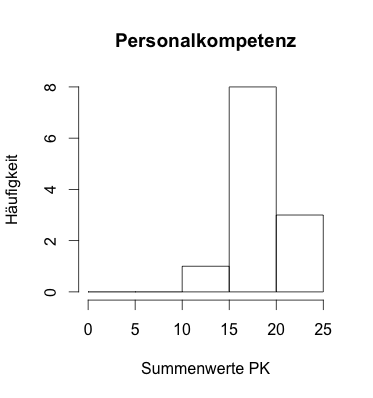
\includegraphics[width=0.33\textwidth]{Anhang/Persohist.png}
\end{figure}

\begin{itemize}
\tightlist
\item
  Kommunikationskompetenz
\end{itemize}

\begin{table}[H]
\centering
\caption{Häufigkeitstabelle Kommunikationskompetenz}
\begin{tabular}{rrrr}
  \hline
 & absolut & Prozent & kumuliert \\
  \hline
(0,4] & 0.00 & 0.00 & 0.00 \\
  (4,8] & 1.00 & 8.33 & 8.33 \\
  (8,12] & 5.00 & 41.67 & 50.00 \\
  (12,16] & 4.00 & 33.33 & 83.33 \\
  (16,20] & 2.00 & 16.67 & 100.00 \\
   \hline
\end{tabular}
\end{table}

\begin{figure}[H]
\centering
\caption{Histogramm Kommunikationskompetenz}
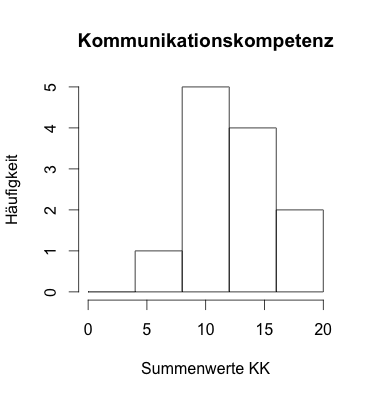
\includegraphics[width=0.33\textwidth]{Anhang/KKHist.png}
\end{figure}

\begin{itemize}
\tightlist
\item
  Nutzungsverhalten
\end{itemize}

\begin{table}[H]
\centering
\caption{Nutzungsverhalten}
\begin{tabular}{rrrr}
  \hline
 & absolut & Prozent & kumuliert \\
  \hline
(0,10] & 1.00 & 8.33 & 8.33 \\
  (10,20] & 10.00 & 83.33 & 91.67 \\
  (20,30] & 1.00 & 8.33 & 100.00 \\
  (30,40] & 0.00 & 0.00 & 100.00 \\
   \hline
\end{tabular}
\end{table}

\begin{figure}[H]
\centering
\caption{Histogramm Nutzungsverhalten}
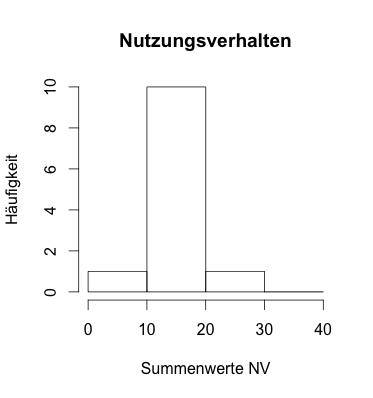
\includegraphics[width=0.33\textwidth]{Anhang/NVHist.png}
\end{figure}

\begin{itemize}
\tightlist
\item
  Handlungskompetenz
\end{itemize}

\begin{table}[H]
\centering
\caption{Häufigkeitstabelle Handlungskompetenz}
\begin{tabular}{rrrr}
  \hline
 & absolut & Prozent & kumuliert \\
  \hline
(0,22.5] & 0.00 & 0.00 & 0.00 \\
  (22.5,45] & 1.00 & 8.33 & 8.33 \\
  (45,67.5] & 6.00 & 50.00 & 58.33 \\
  (67.5,90] & 5.00 & 41.67 & 100.00 \\
   \hline
\end{tabular}
\end{table}

\begin{figure}[H]
\centering
\caption{Histogramm Handlungskompetenz}
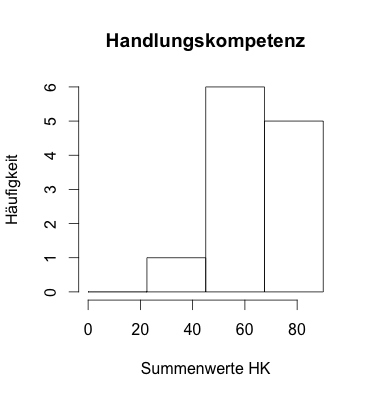
\includegraphics[width=0.33\textwidth]{Anhang/HKHist.png}
\end{figure}

\begin{table}[H]
\centering
\caption{Gesamtkompetenz und Nutzungsverhalten}
\begin{tabular}{rr}
  \hline
 Parameter & Mittelwerte\\
  \hline
Gesamtscore.Kompetenzen & 65.58 \\
  Mittelwert.Kompetenzen & 3.60 \\
  Gesamtscore.Nutzungsverhalten & 16.42 \\
  Mittelwert.Nutzungsverhalten & 2.05 \\
  Gesamtscore.passive.Nutzung & 10.17 \\
  Mittelwert.passive.Nutzung & 2.54 \\
  Gesamtscore.aktive.Nutzung & 6.25 \\
  Mittelwert.aktive.Nutzung & 1.56 \\
   \hline
\end{tabular}
\end{table}

\pagebreak

\pagebreak
\printbibliography
\pagebreak
\appendix


  \section{Anhang}
  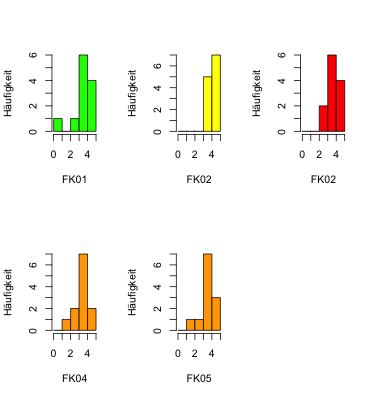
\includegraphics{Anhang/schoen.png}
  %\subsection{Abkürzungen}
  %\renewcommand{\thetable}{{A}.\arabic{table}}
  %\renewcommand{\thetable}{\Alph{section}.\arabic{table}}
  \begin{table}[H]
\centering
%\captionof{table}[Anhang]{Titel}
%\caption{Zuordnung der Items}
\label{itemtabelle}
\resizebox{\textwidth}{!}{%
\begin{tabular}{@{}lllll@{}}
\toprule
Item  & Konstrukt                                                                    & Indikator                                                                                                                                                                           & Ausprägung                                                                                                                                                                                       & Skalenniveau \\ \midrule
1-5   & \begin{tabular}[c]{@{}l@{}}Fach-\\ kompetenz\\FK1,FK2,FK3,FK4,FK5\end{tabular}                    & \begin{tabular}[c]{@{}l@{}}Disposition sachlich-gegenständliche\\ Probleme selbstorganisiert lösen zu können\end{tabular}                                                           & \begin{tabular}[c]{@{}l@{}}5-stufige Likertskala:\\ 1= trifft überhaupt nicht zu\\ 2= trifft wenig zu\\ 3=trifft teils/teils zu\\ 4=trifft überwiegend zu\\ 5=trifft völlig zu\end{tabular}      & metrisch     \\
\midrule
6-10  & \begin{tabular}[c]{@{}l@{}}Methoden-\\ kompetenz\\MK1,MK2,MK3,MK4\end{tabular}                & \begin{tabular}[c]{@{}l@{}}Tätigkeiten und Aufgaben methodisch\\  selbst-organisiert zu gestalten und Methoden\\  weiter zu entwickeln\end{tabular}                                 & \begin{tabular}[c]{@{}l@{}}5-stufige Likertskala: \\ 1= trifft überhaupt nicht zu\\ 2= trifft wenig zu \\ 3=trifft teils/teils zu \\ 4=trifft überwiegend zu \\ 5=trifft völlig zu\end{tabular}  & metrisch     \\
\midrule
11-16 & \begin{tabular}[c]{@{}l@{}}Personal-\\ kompetenz\\PK1,PK2,PK3,PK4,PK5\end{tabular}                & \begin{tabular}[c]{@{}l@{}}Sich einschätzen, selbstorganisiert reflexiv\\  handeln,Werte, Motive und Selbstbilder\\  entwickeln\end{tabular}                                        & \begin{tabular}[c]{@{}l@{}}5-stufige Likertskala: \\ 1= trifft überhaupt nicht zu \\ 2= trifft wenig zu \\ 3=trifft teils/teils zu \\ 4=trifft überwiegend zu \\ 5=trifft völlig zu\end{tabular} & metrisch     \\
\midrule
17-21 & \begin{tabular}[c]{@{}l@{}}Komunikations-\\ kompetenz\\KK1,KK2,KK3,KK4\end{tabular}           & \begin{tabular}[c]{@{}l@{}}Sich mit anderen kreativ auseinander setzen, \\ kommunikativ und selbstorganisiert handeln\\ \parencite[8]{ErpenbeckRosenstiel200305}\end{tabular} & \begin{tabular}[c]{@{}l@{}}5-stufige Likertskala\\ 1= trifft nicht zu,\\2= trifft wenig zu \\ 3=trifft teils/teils zu \\ 4=trifft überwiegend zu \\ 5=trifft vollständig zu\end{tabular}                                                                                    & metrisch     \\
 \midrule
22-28 & \begin{tabular}[c]{@{}l@{}}Nutzungs\\ verhalten\\ Lernplattform NV1,NV2,NV3\\NV4,NV5,NV6,NV7,NV8\end{tabular} & \begin{tabular}[c]{@{}l@{}}Aufschluss über die Intensität u\\ der Nutzung der Lernplattform\end{tabular}                                                                 & \begin{tabular}[c]{@{}l@{}}5-stufige Skala\\ 1=0-1mal genutzt\\ 2=2-4 mal genutzt\\ 3=5-7 mal genutzt\\ 4=8-10 mal genutzt\\ 5=\textgreater10 mal genutzt\end{tabular}                            & metrisch     \\ \bottomrule
\end{tabular}%
}
\end{table}



%\input{tabelleanalysen}
%\includepdf{alleine.pdf}
\end{document}
